%===========================================================
%                              Choix: RenPar / SympA / CFSE
%===========================================================
% Une des trois options 'renpar', 'sympa' et 'cfse' doit
% être utilisée avec le style compas2013 en fonction 
% de l' l'appel à soumission choisi.
\documentclass[renpar]{compas2013}
\usepackage{todonotes}
\usepackage{listings}

\usepackage{tikz}
\usetikzlibrary{positioning}
\usetikzlibrary{arrows}
\usetikzlibrary{calc}
\usetikzlibrary{backgrounds}
\usetikzlibrary{trees}
\usetikzlibrary{shadows}

%===========================================================
%                               Title
%===========================================================

\toappear{1} % Conserver cette ligne pour la version finale

\begin{document}

\title{Pythran~: Génération automatique de modules natifs parallèles à
partir de modules Python avec annotations OpenMP}
\shorttitle{Génération automatique de modules natifs parallèles pour
Python}

\author{Serge \textsc{Guelton}}%\thanks{Le texte a été relu par Thierry Gautier.}%

\address{École Normale Supérieure,\\
Département d'informatique\\
45 rue d'Ulm, F-75230 Paris Cedex 05 -- France\\
serge.guelton@telecom-bretagne.eu}

\date{6 septembre 2012}

\maketitle

%===========================================================         %
%Résumé
%===========================================================  
\begin{abstract}
  Cet article étudie l'utilisation des directives OpenMP dans le cadre de
  programmes écrits en Python. La méthode proposée est de traduire le
  code Python annoté en un code C++ conservant les annotations.
  
  L'approche est mise en pratique dans le compilateur pythran, qui est
  capable de compiler statiquement un module écrit dans un sous-ensemble
  statiquement typé du langage Python et annoté de directives OpenMP en un
  module natif dont certaines sections de code s'exécutent en parallèle. 

  On peut ainsi générer des modules dont les temps d'exécutions sont 100
  fois inférieurs à ceux du module d'origine, grâce à la compilation
  statique et à l'utilisation du parallélisme.
  
  \MotsCles{Python, OpenMP, C++}
\end{abstract}

	
%=========================================================
\section{Introduction}
%=========================================================

Le langage Python~\cite{rossum97} est né en décembre 1989. Depuis, son
caractère extrêmement dynamique, sa bibliothèque standard riche, son large
écosystème et sa syntaxe concise lui ont permis de toucher de nombreux
domaines d'applications, dont par exemple l'administration système ou les
services webs.  Python a également percé dans le monde du calcul
scientifique~\cite{Oliphant2007}, notamment grâce au paquet
SciPy~\cite{scipy}. Le surcout d'interprétation du langage Python étant
rédhibitoire pour une utilisation dans un contexte de calcul intensif,
SciPy repose sur deux concepts pour atteindre un bon niveau de
performance~: les noyaux de calculs intensifs sont écrits dans des
langages de bas niveau, C et Fortran, dont les appels sont encapsulés par
un module dit \emph{natif}~; et la structure de données de base, le
tableau multidimensionnel~\cite{numpyarray2011} a été conçue pour être
accessible à la fois par les modules natifs et l'interpréteur Python sans
surcout de conversion.

Pour faciliter l'écriture par l'utilisateur de modules natifs, c'est à
dire sans avoir à écrire soi-même le code permettant de traduire des
objets Python en structures natives et d'appeler une fonction C depuis
l'interpréteur, le paquet SciPy fournit le module \texttt{weave} qui
permet d'intégrer de petits fragments de code C à un module python, ce
code étant par la suite compilé et chargé dynamiquement à l'exécution,
pour des temps d'exécution moindres.

Cette approche hybride, consistant à mélanger code interprété et code
compilé dans un même flot d'exécution, est présente sous de nombreuses
formes dans le paysage Python. La Section~\ref{sec:python-hybrid} étude
les différentes approches qui ont été explorées et montre le manque de
support du parallélisme dans ces approches. La
Section~\ref{sec:python-parallelism} fournit des éléments d'explications à
ce phénomène et propose l'ajout du support des directives OpenMP au langage
dans le cadre d'un \emph{domain specific language} embarqué dans Python et
compilable statiquement, Pythran. Ce langage et les contraintes qu'il doit
respecter pour être compilable statiquement et compatible avec la norme
OpenMP sont exposés à la Section~\ref{sec:pythran}. Un compilateur pour ce
langage a été écrit et a permis de mesurer des temps d'exécutions
significativement inférieur à ceux obtenus avec l'implémentation de
référence de l'interpréteur Python, comme présenté en
Section~\ref{sec:validation}.

%=========================================================
\section{Systèmes hybrides en Python}\label{sec:python-hybrid}
%=========================================================

Dans le cadre qui nous intéresse, un système hybride où une partie du code
spécifié par l'utilisateur est exécutée par l'interpréteur Python et une
partie est exécutée nativement, comme introduit dans~\cite{dongara2007}.

Il est possible d'écrire des modules natifs directement en langage C/C++.
Il faut dans ce cas respecter l'interface fournie dans~\cite{pythoncapi},
ce qui conduit à l'écriture d'une quantité non négligeable de code
d'encapsulation. Des outils ont été développé pour réduire ce coût de
développement, notamment Swig~\cite{swig2003} qui utilise un fichier
d'interface spécifique pour guider la traduction, et
\texttt{boost::python}~\cite{boostpython2007} qui se base lui sur le
langage C++ pour guider la traduction.

Une approche concurrente est de se baser sur le langage hôte --- ici
Python --- pour décrire les deux parties du système, et de laisser un
outil tierce convertir une partie de l'application en code natif,
généralement la partie la plus demandeuse en ressources de calcul.
L'avantage est de permettre à des développeurs qui ne seraient pas
familiers avec les langages C/C++ ou qui n'auraient pas de temps à
consacrer à écrire une partie de leur application dans ces langages,
d'obtenir des performances satisfaisantes avec un investissement moindre.
Cette approche a fait l'objet de nombreuses études et solutions
techniques, que l'on peut classifier suivant leur caractère intrusif ou
non et sur le support de toute ou partie des fonctionnalités du langage.

\subsection{Approches intrusives}

Un des points contraignants du langage Python est son typage structurel
implicite. Il implique par exemple que chaque appel de méthode est résolu
dynamiquement. Il n'est alors pas surprenant que de nombreuses approches
s'attachent à l'annotation de code Python pour y apporter une couche de
typage statique, mais aussi pour typer les types flottants en entier plus
finement que les trois options fournies par Python, entiers 64 bits,
entiers multi-précision et nombres flottants double précision. Ainsi
cython~\cite{cython2010} propose un dialecte de Python permettant de
convertir un module Python fortement annoté à l'aide de types C ou d'appel
de fonctions natives. plw~\cite{dongara2007} propose une approche
similaire, en limitant la conversion à des portions de code délimitées par
des annotations, et en générant du C++. Le projet
numba~\footnote{\emph{cf}.\ \texttt{https://github.com/numba/numba}}
fonctionne sur le même principe, mais en générant du code LLVM.

\subsection{Approches non-intrusives}

Le problème des approches intrusives et qu'elles impliquent de modifier du
code existant de façon non bénigne, et demandent l'investissement dans un
nouveau langage, investissement dont la pérennité n'est pas toujours
garantie. \emph{A contrario} les approches non-intrusives, si elles
contraignent éventuellement le langage d'entrée, n'ajoutent pas de
nouvelles constructions et restent compatibles avec l'interpréteur 

L'interpréteur PyPy~\cite{pypy2009}, lui-même écrit en Python, vise à
supporter la totalité du langage Python. Il utilise un JIT traceur qui
génère du code natif ---sans passer par un compilateur intermédiaire ---
pour les points chauds.

Le compilateur shedskin~\cite{shedskin2006} traduit du Python en C++. Il
pose néanmoins plusieurs contraintes sur le code d'entrée~: absence de
n-uplets, pas de variables polymorphes et pas d'introspection. De nombreux
modules de la bibliothèque standard sont supportés. La traduction se fait
pour un programme complet ou par module.

Le compilateur copperhead~\cite{copperhead2011} traduit quant à lui un DSL
embarqué dans Python, se limitant ainsi à un sous-ensemble en assignation
unique autorisant tableaux et n-uplets et restreignant énormément le flot
de contrôle (ni boucles, ni exceptions\dots). En contrepartie, ce DSL est
automatiquement parallélisé et traduit en CUDA ou C++ avec appels à la
bibliothèque Thrust~\footnote{\emph{cf}.\
\texttt{http://thrust.github.com/}}. La traduction se fait dynamiquement
pour les fonctions identifiées par un décorateur spécifique.

Seul copperhead permet de générer des modules natifs parallèles, mais
l'expressivité de ce langage ne lui permet que de toucher une petite
classe d'applications. La section suivante étudie les limitations de
Python vis-à-vis du parallélisme et conduit à une proposition originale
visant à pallier ses limitations.

%=========================================================
\section{Python et Parallélisme}\label{sec:python-parallelism}
%=========================================================

La parallélisation de langage de scripts est une approche naturelle pour
compenser leur manque relatif de performance. L'étude menée
dans~\cite{choy05} montre les nombreuses approches explorées autour du
langage MATLAB. Une approche purement automatique pour le langage R est
décrite dans~\cite{mals07}. Peu de travaux traitent du langage Python et
de ses spécificités.

\subsection{Python et processus lourds}

La parallélisation de calculs est supportée en Python à travers le module
\texttt{multiprocessing} fourni dans la bibliothèque standard.  Il permet
de piloter différent processus fils en mode client-serveur. La
communication entre processus se fait par queue ou pile en utilisant la
sérialisation native des objets. Il est également possible de partager des
segments mémoire. Cette approche est adaptée pour du parallélisme gros
grains, mais est moins importante qu'une approche basée sur des processus
légers communiquant par mémoire partagée pour du parallélisme à grain fin.

\subsection{Python et processus légers}

Le langage Python offre la capacité de démarrer plusieurs processus légers
dans le même interpréteur. Cependant, ce type de parallélisation n'est pas
adapté au calcul intensif en raison d'un mécanisme propre à CPython,
l'implémentation de référence de l'interpréteur: le \emph{Global
Interpreter Lock}~\cite{gil2012}~\footnote{D'autres implémentations, comme
IronPython et Jython, ne souffrent pas de cette limitation.}. Ce verrou
est utilisé, entre autres, par le ramasse-miette et il est pris à chaque
appel de méthode d'un objet.  Certains modules reposent également sur ce
verrou pour garantir certains invariants. Ce verrou rend impossible
l'utilisation de processus légers pour du calcul scientifique.

\subsection{Proposition}

Les développeurs Python désirant utiliser des machines multi-cœurs
utilisent souvent des modules natifs au sein desquels ils peuvent utiliser
des processus légers sans être contraints par le GIL. On obtient ainsi le
double intérêt d'un module natif et d'un module parallèle.

Cet article propose d'automatiser cette approche en~:
\begin{enumerate}
  \item donnant la possibilité d'annoter du code Python avec des
	directives OpenMP~\cite{openmp3.1};
  \item convertissant ce code Python en code C++11~\cite{isocxx11} en conservant la
	sémantique des annotations.
\end{enumerate}


%=========================================================
\section{Pythran}\label{sec:pythran}
%=========================================================

\subsection{Support d'OpenMP en Python}
\label{sec:python-openmp}

\subsubsection{Ajout des annotations}

Le langage Python permet de faire porter des annotations par des
fonctions, sous la forme de décorateurs. Aucun mécanisme n'est prévu pour
décorer des instructions. Une approche possible est d'utiliser des
commentaires, à la manière de l'intégration d'OpenMP dans le langage
FORTRAN. Cependant, le module \texttt{ast} de la bibliothèque standard,
qui fournit une API pour l'analyse lexicale et syntaxique du langage, ne
conserve pas les commentaires. Une alternative satisfaisante consiste
alors à interpréter les instructions ne comprenant qu'une expression de type
chaîne de caractères comme une annotation portant sur l'instruction
suivant directement. Par exemple, on pourra écrire~:

\begin{lstlisting}[language=python]
"omp parallel for reduction(r), private(auto)"
for auto in mon_conteneur:
  r+=x
\end{lstlisting}

Il est dangereux de représenter les annotations sous forme de chaîne de
caractères, car elles font éventuellement référence à des variables du
programme, par exemple \texttt{auto} dans l'exemple précédent, qui peuvent
être amenés à être renommée dans le flot de compilation.

L'arbre de syntaxe abstrait fourni par le module \texttt{ast} est alors
étendu en ajoutant un attribut \texttt{annotation} à toutes les
instructions~:

\begin{lstlisting}
annotation(str description, Name* identifiers)
\end{lstlisting}

\noindent où \texttt{description} est une chaîne de caractère décrivant
l'annotation et paramétrée par la liste d'indentifiants
\texttt{identifiers}. Le type \texttt{Name} est la façon canonique de
représenter un identifiant dans le module \texttt{ast}.  En opérant de la
sorte, toutes les opérations de renommage pourront utiliser un visiteur
générique spécialisé pour le type \texttt{Name}.

\subsubsection{Spécificités liées à Python}

À la manière de FORTRAN, le langage Python ne permet pas de créer des
blocs structurés sur lesquels l'on pourrait faire porter une annotation.
Le problème est résolu en FORTRAN en utilisant des commentaires pour
délimiter les débuts et fin de bloc. Cette solution ne se conforme pas aux
canons du langage, on lui préfèrera l'extraction du bloc concerné dans une
nouvelle fonction.

Il n'existe en Python que des variables locales à une fonction, non pas à
un bloc. Cela à une influence sur le mode de partage des variables à
l'intérieur, par exemple, d'une boucle parallèle. Dans le code suivant~:

\begin{lstlisting}[language=python]
for x in mon_conteneur:
  f=foo(x)
  b=bar(x)
  r+=f*b
\end{lstlisting}

\noindent l'instruction \texttt{for} référence les variables \texttt{x},
\texttt{mon\_conteneur}, \texttt{f}, \texttt{b} et \texttt{r} en plus des
appels de fonction. Le mode de partage par défaut de ses variables est
\texttt{shared}, il faut donc lister \emph{toutes} les variables privées
dans une clause \texttt{private} pour obtenir un bon degré de parallélisme.

À titre d'exemple, le Listing~\ref{lst:pythran-mat-mul} illustre une
multiplication de matrices annotées par des directives OpenMP.

\begin{lstlisting}[language=python, label={lst:pythran-mat-mul},caption={multiplication de matrice avec
  annotations OpenMP}]
def zero(n,m): return [[0 for row in xrange(n)] for col in xrange(m)]
def matrix_multiply(m0, m1):
  new_matrix = zero(len(m0),len(m1[0]))
  "omp parallel for private(i,j,k)"
  for i in xrange(len(m0)):
    for j in xrange(len(m1[0])):
      for k in xrange(len(m1)):
        new_matrix[i][j] += m0[i][k]*m1[k][j]
  return new_matrix
\end{lstlisting}


\subsection{Organisation de Pythran}

Le fonctionnement du compilateur Pythran est détaillé à la
Figure~\ref{fig:pythran}. L'outil convertit un module python complet,
éventuellement annoté de directives OpenMP et avec des indications de
types pour les fonctions exportées par le module. Il transforme le tout en
code C++11 annoté, qui, lié avec un environnement d'exécution nommé
\texttt{pythonic++} et l'encapsulation fournie par \texttt{boost::python},
conduit à un module natif.

\begin{figure}
  \centering
  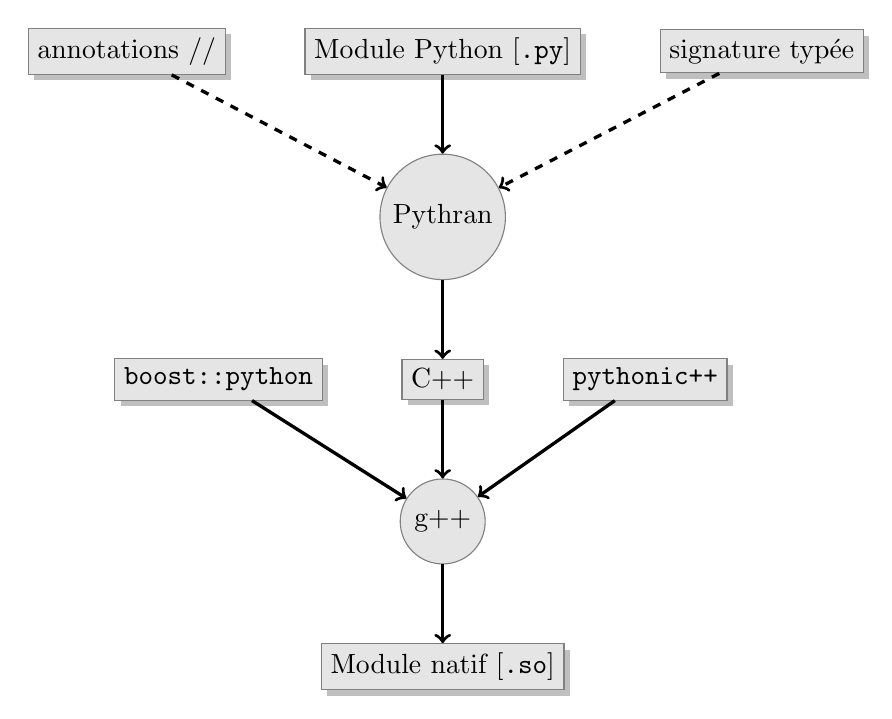
\begin{tikzpicture}[
	file/.style={draw=black!50,fill=black!10,rectangle, drop shadow, align=center},
	tool/.style={draw=black!50,fill=black!10,circle, align=center}]
	\node[file] (python) {Module Python [\texttt{.py}]};
	\node[file] (annotation)	   [right=of python] {signature typée};
	\node[file] (omp)	   [left=of python] {annotations //};
	\node[tool] (pythran) [below=of python] {Pythran};
	\node[file] (cxx) [below=of pythran] {C++};
	\node[file] (boost) [left=of cxx] {\texttt{boost::python}};
	\node[file] (pythonic) [right=of cxx] {\texttt{pythonic++}};
	\node[tool] (gxx) [below=of cxx] {g++};
	\node[file] (so) [below=of gxx] {Module natif [\texttt{.so}]};

	\draw[very thick, ->] (python) -- (pythran);
	\draw[very thick,dashed, ->] (annotation) -- (pythran);
	\draw[very thick,dashed, ->] (omp) -- (pythran);
	\draw[very thick, ->] (pythran) -- (cxx);
	\draw[very thick, ->] (cxx) -- (gxx);
	\draw[very thick, ->] (boost) -- (gxx);
	\draw[very thick, ->] (pythonic) -- (gxx);
	\draw[very thick, ->] (gxx) -- (so);
  \end{tikzpicture}

  \caption{Fonctionnement schématique du compilateur Pythran}
  \label{fig:pythran}
\end{figure}

Le flot de compilation utilisé en interne par Pythran peut être modélisé de la façon
suivante~:

\begin{enumerate}
  \item\label{enum:lex-yacc} analyse lexicale \& syntaxique~;
  \item\label{enum:openmp} intégration des directives OpenMP~;
  \item\label{enum:simplification-ast} simplification de l'arbre de syntaxe abstrait~;
  \item\label{enum:typage-ast} typage paramétrique de l'arbre de syntaxe abstrait~;
  \item\label{enum:instanciation-types} instanciation des types paramétriques~;
  \item\label{enum:traduction-cxx} traduction de la représentation Python en une représentation C++~;
  \item\label{enum:compilation-extrene} compilation par un compilateur externe en une bibliothèque
	partagée.
\end{enumerate}

Ces différentes étapes sont décrites par la suite, à l'exception de
l'item~\ref{enum:lex-yacc}, et de l'item~\ref{enum:openmp} déjà discuté en
Section~\ref{sec:python-openmp}.

\subsubsection{Simplification de la grammaire}

Le langage Pythran supporte un sous ensemble de la grammaire du langage
Python. Les mots clés \texttt{class} et \texttt{exec} ne sont pas
supportés~\footnote{D'autres constructions, telles les variables globales
ou les gestionnaires de contexte à l'aide du mot-clé \texttt{with} ne sont
pas supportés, mais cela est plus lié à des priorités de développement
qu'à des problèmes fondamentaux.}. L'absence de classe utilisateur
simplifie l'inférence de type et la gestion de la mémoire. Plusieurs
classes natives, notamment tous les conteneurs, sont supportées.
L'évaluation dynamique de chaîne de caractère comme code source ne rentre
pas dans les possibilités du langage cible. De même, certaines fonction
intrinsèques telles \texttt{eval} ne sont pas supportées. Le langage
intermédiaire utilisé par PyPy, RPython~\cite{rpython2007}, est soumis à
des contraintes de staticité similaires.

Une fois que la validité de la syntaxe est assurée, l'arbre de syntaxe
abstrait est transformé en un nouvel arbre.
\begin{enumerate}

  \item Les fonctions anonymes sont transformées en fonctions imbriquées~:
	\texttt{lambda x:a*x} devient \texttt{def foo(x): return a*x}.

  \item Les fonctions imbriquées, utilisant des fermetures, sont
	transformées en fonctions globales prenant leur contexte en
	paramètre~: \texttt{def foo(x): return a*x} devient \texttt{def
	foo(a,x): return a*x}.

  \item Les listes/ensembles/dictionnaires en compréhension sont
	transformés en appels de fonction faisant apparaître explicitement la
	structure de boucle~:\texttt{[x*x for x in l]} devient
\begin{lstlisting}[language=python]
def foo(y):
	tmp=list()
	for x in y: tmp.append(x*x)
	return tmp
foo(l)
\end{lstlisting}

  \item Les attributs de classe sont transformés en indices constants~:
	\texttt{c.real+c.imag} devient \texttt{c[0]+c[1]}.

  \item Les appels de méthodes sont transformés en appels de fonctions~:
	\texttt{l.append(v)} devient \texttt{any.append(l,v)}.

  \item Les valeurs de retour implicites sont rendus
	explicites~\footnote{Toute fonction Python a une valeur de retour, qui
	se trouve être \texttt{None} par défaut.}:\texttt{def foo(): print
	"bar"} devient \texttt{def foo(): print "bar" ; return None}.

  \item Tous les symboles importés de manière relative sont remplacés par
	leur chemin absolus~: \texttt{from math import cos as COS ; COS(3)}
	devient \texttt{import math ; math.cos(3)}.

\end{enumerate}

Ces étapes de raffinement conduisent à une représentation interne à
Pythran plus concise et facile à manipuler que l'arbre de syntaxe abstrait
de Python. 

Un point crucial à respecter lors de ces transformations d'arbre est de
garantir la validité de ces transformations vis-à-vis des annotations
OpenMP portées par les instructions. Comme le compilateur Pythran n'a pas
de compréhension directe du sens de l'annotation, il garantit qu'une
annotation est toujours attachée à la même instruction, et qu'au cas où
une instruction devait être transformée en plusieurs, l'annotation serait
portée par le bloc d'instructions crée. Par exemple~:
%
\begin{lstlisting}[language=python]
"omp critical"
a,b=make_tuple()
\end{lstlisting}
%
\noindent peut être transformé en
\begin{lstlisting}[language=python]
"omp critical"
if 1:
	t=make_tuple()
	a=t[0] ; b=t[1]
\end{lstlisting}
%
\noindent afin de conserver l'annotation.

\subsubsection{Typage}

Pythran utilise une variante de l'algorithme d'inférence de type de
Hindley--Milner~\cite{milner78}. À l'issu de son application, tous les
nœuds de la représentation interne se voient dotés d'un type paramétrique,
dépendant du type symbolique de ses paramètres.

L'instanciation des types paramétriques est déclenchée par une annotation
fournie par l'utilisateur, qui spécifie la signature des fonctions
exportées par le module sous la forme~:
%
\begin{lstlisting}[language=python]
#pythran export matrix_multiply(int list list, int list list)
#pythran export matrix_multiply(float list list, float list list)
\end{lstlisting}
%
Plusieurs annotations pour la même fonction peuvent coexister~: plusieurs
fonctions sont alors générées.

Cet article ne vise pas à expliquer en détail le fonctionnement de cette
étape. On admettra donc que cette analyse permet à Pythran d'accepter des
fonctions polymorphes, mais uniquement des variables monomorphes.

Pour faciliter la gestion de la mémoire, on ajoute une nouvelle
contrainte~: il ne peut y avoir de dépendance circulaire dans la
définition des types des objets. Ce genre de dépendance ne pause aucun
problème en Python, et demande l'utilisation de pointeurs en C/C++.


\subsubsection{Gestion de la mémoire}

En Python, une instance de classe est accessible via sa référence. Une
affectation est une copie de référence, et non pas de l'objet lui-même.
L'implémentation de référence, CPython, gère la mémoire en utilisant deux
stratégies~:compteurs de référence et ramasse-miette.

La première stratégie peut être employée --- avec un certain coût --- en
C++ par l'utilisation de pointeurs partagés, les \texttt{std::shared\_ptr}
disponible dans la bibliothèque standards.  Grâce à la contrainte sur
l'absence de dépendances de type circulaires, le comptage de référence est
un mécanisme suffisant pour garantir l'absence de fuites de mémoires. De
plus, il garantit une libération «~au plus tôt~» des ressources.

Cependant, l'utilisation de compteurs partagés dans un contexte parallèle,
implique de prendre un certain nombre de précautions. Pythran utilise pour
le moment un simple verrou, mais des techniques plus performantes ont été
développées par ailleurs~\cite{Levanoni2006}.

%=========================================================
\section{Validation et expériences}\label{sec:validation}
%=========================================================

\subsection{Validation}

La vérification de la validité de la traduction effectuée par Pythran
repose sur des test unitaires, constitués d'une fonction et de ses
arguments.  Cette fonction est généralement courte, elle retourne une
valeur servant de trace et est déterministe.

Pour chaque test unitaire, la fonction correspondante est exécutée par
l'interpréteur avec les arguments fournis et sa valeur de retour est
mémorisée. La même fonction est alors compilée par Pythran en un module
natif qui est ensuite chargé dynamiquement dans l'interpréteur pour être
exécuté avec les mêmes arguments pour récupérer une nouvelle trace. Le
test est considéré comme valide si les deux traces sont identiques. On
garantit ainsi le même comportement entre les deux versions.

En plus des test unitaires, des applications complètes sont utilisées pour
comparer les performances du code compilé à celles de l'interpréteur.

\subsection{Mesures de performances}

Les mesures faites ici comparent les temps d'exécution de plusieurs
applications exécutées par les interpréteurs CPython ou par PyPy, ou après
transformation en un module natif par les traducteurs Shedskin et Pythran.

Les codes utilisés sont tirés des bases de tests du défunt projet
\texttt{unladen swallow}, ou issus de la littérature. La seule
modification faite est l'ajout de la signature typée de la fonction
appelée. Quand cela était possible, des annotations OpenMP ont été
ajoutée. \texttt{extrema} recherche les valeurs extrêmes d'une liste,
\texttt{matmul} effectue une produit matriciel entre deux matrices
carrées, \texttt{mandel} fait un calcul de fractal, \texttt{nqueens}
résout une instance du problème des n-reines, \texttt{pi\_buffon} utilise
une méthode de monte-carlo pour calculer les décimales de $\pi$,
\texttt{quicksort} est une implémentation récursive du tri rapide et
\texttt{stone} est l'adaptation en Python du vénérable test de
performances \texttt{wetstone}.

Toutes les mesures de temps sont faites à l'aide du module
\texttt{timeit}. Elles représentent le temps d'exécution médian sur 100
itérations. Les mesures \emph{incluent} le coût de conversion entre les
structures de données Python et leur représentation native.

Les évaluations de performances sont effectuées sur une machine comportant
4 processeurs de type Intel Core i7 avec l'\emph{hypethreading}, avec 8G
de RAM et tournant un noyau 3.0.0.
Les modules Pythran sont compilés avec g++-4.7.1 et les drapeaux
\texttt{-Ofast -DNDEBUG}.
Les temps reproduits ici sont obtenus à l'aides des commandes
\texttt{python setup.py bench} et \texttt{python setup.py bench
--parallel} fournie avec l'installation de Pythran.

Le tableau~\ref{tbl:pythran-vs-cpython} illustre les performances de
Pythran par rapport à CPython, en prenant en compte ou non les directives
OpenMP. Il permet d'observer des gains importants dus au changement de
langage. On observe aussi que les directives OpenMP sont bien prises en
compte et permettent d'obtenir des facteurs d'accélération du module natif
parallèle allant jusqu'à $\times300$ par rapport à CPython et $\time8$ par
rapport à PyPy.

\begin{table}
  \begin{tabular}{|l|c|c|c|c|}
				&CPython	&	PyPy	&	Pythran	&	Pythran+OpenMP\\
	nqueens		&1.754		&	0.603	&	0.228	&	0.231		  \\
	pi\_buffon	&47.083		&	12.08	&	2.676	&	0.561		\\
	extrema		&0.386		&	0.564	&	0.033	&	0.033\\
	stone		&6.956		&	0.204	&	0.023	&	0.023\\
	mandel		&976.81		&	6.304	&	5.563	&	2.565\\
	caxpy		&0.588		&	0.204	&	0.340	&	0.340\\
	matmul		&153.91		&	9.061	&	7.314	&	2.263\\
	quicksort	&3.331		&	0.087	&	0.040	&	0.041\\
  \end{tabular}

  \caption{Comparaison de CPython, PyPy et Pythran, avec ou sans OpenMP.}
  \label{tbl:pythran-vs-cpython}
\end{table}

%=========================================================
\section{Conclusion}
%=========================================================

Cet article présente l'ajout du support OpenMP au langage Python dans le
cadre du traducteur Python vers C++ Pythran. Partant d'un large
sous-ensemble du langage, il propose une syntaxe simple pour annoter des
instructions Python, et un processus de traduction conservatif pour
traduire ses annotations en directives pour le langage C++. Le code généré
repose sur une bibliothèque paramétrique compatible avec une utilisation
en mode parallèle.

Le code généré est évalué pour ses versions séquentielles et parallèles. La
comparaison avec des approches séquentielles existantes montre des gains
de $\times XY$ à $\times YZ$ très encourageants.



%=========================================================
\section{Remerciements}
%=========================================================

L'auteur tient à remercier la société Silkan pour avoir financé une partie des
développements du compilateur Pythran. Il remercie également Albert
\textsc{Cohen} pour lui avoir libéré du temps pour travailler sur ce projet.

Plusieurs discussions avec Pierre \textsc{Fiorini}, Bryan
\textsc{Catanzero}, Joël \textsc{Falcou} et Mathias \textsc{Gaunard} ne
sont pas étrangères aux idées exposées dans cet article.

Les nombreux conseils de Fabien \textsc{Dagnat} ont fortement contribué à
la réflexion sur le typage statique de code Python. Deux élèves de Télécom
Bretagne, Adrien \textsc{Merlini} et Pierrick \textsc{Brunet}, ont apporté
une aide inestimables pour le support des listes, des exceptions et des
ensembles.

\bibliography{biblio}


\end{document}








